\documentclass[a4paper,12pt]{article}

\usepackage{../usfdvl}

\title{Worksheet 2}
\SetDocumentFooter{}{}


\begin{document}

\maketitle

\worksheetGroundRules

\worksheetSubmission


\vspace{5pt}
\section{Assignment}

\vspace{10pt}
\myparagraph{For the line segments below, use the following pages to \uline{show the 8 iterations of the AABB sweep algorithm (w/o the interval tree). At each step show the event queue, interval list, and indicate which segments are compared for intersection.}}


\begin{center}
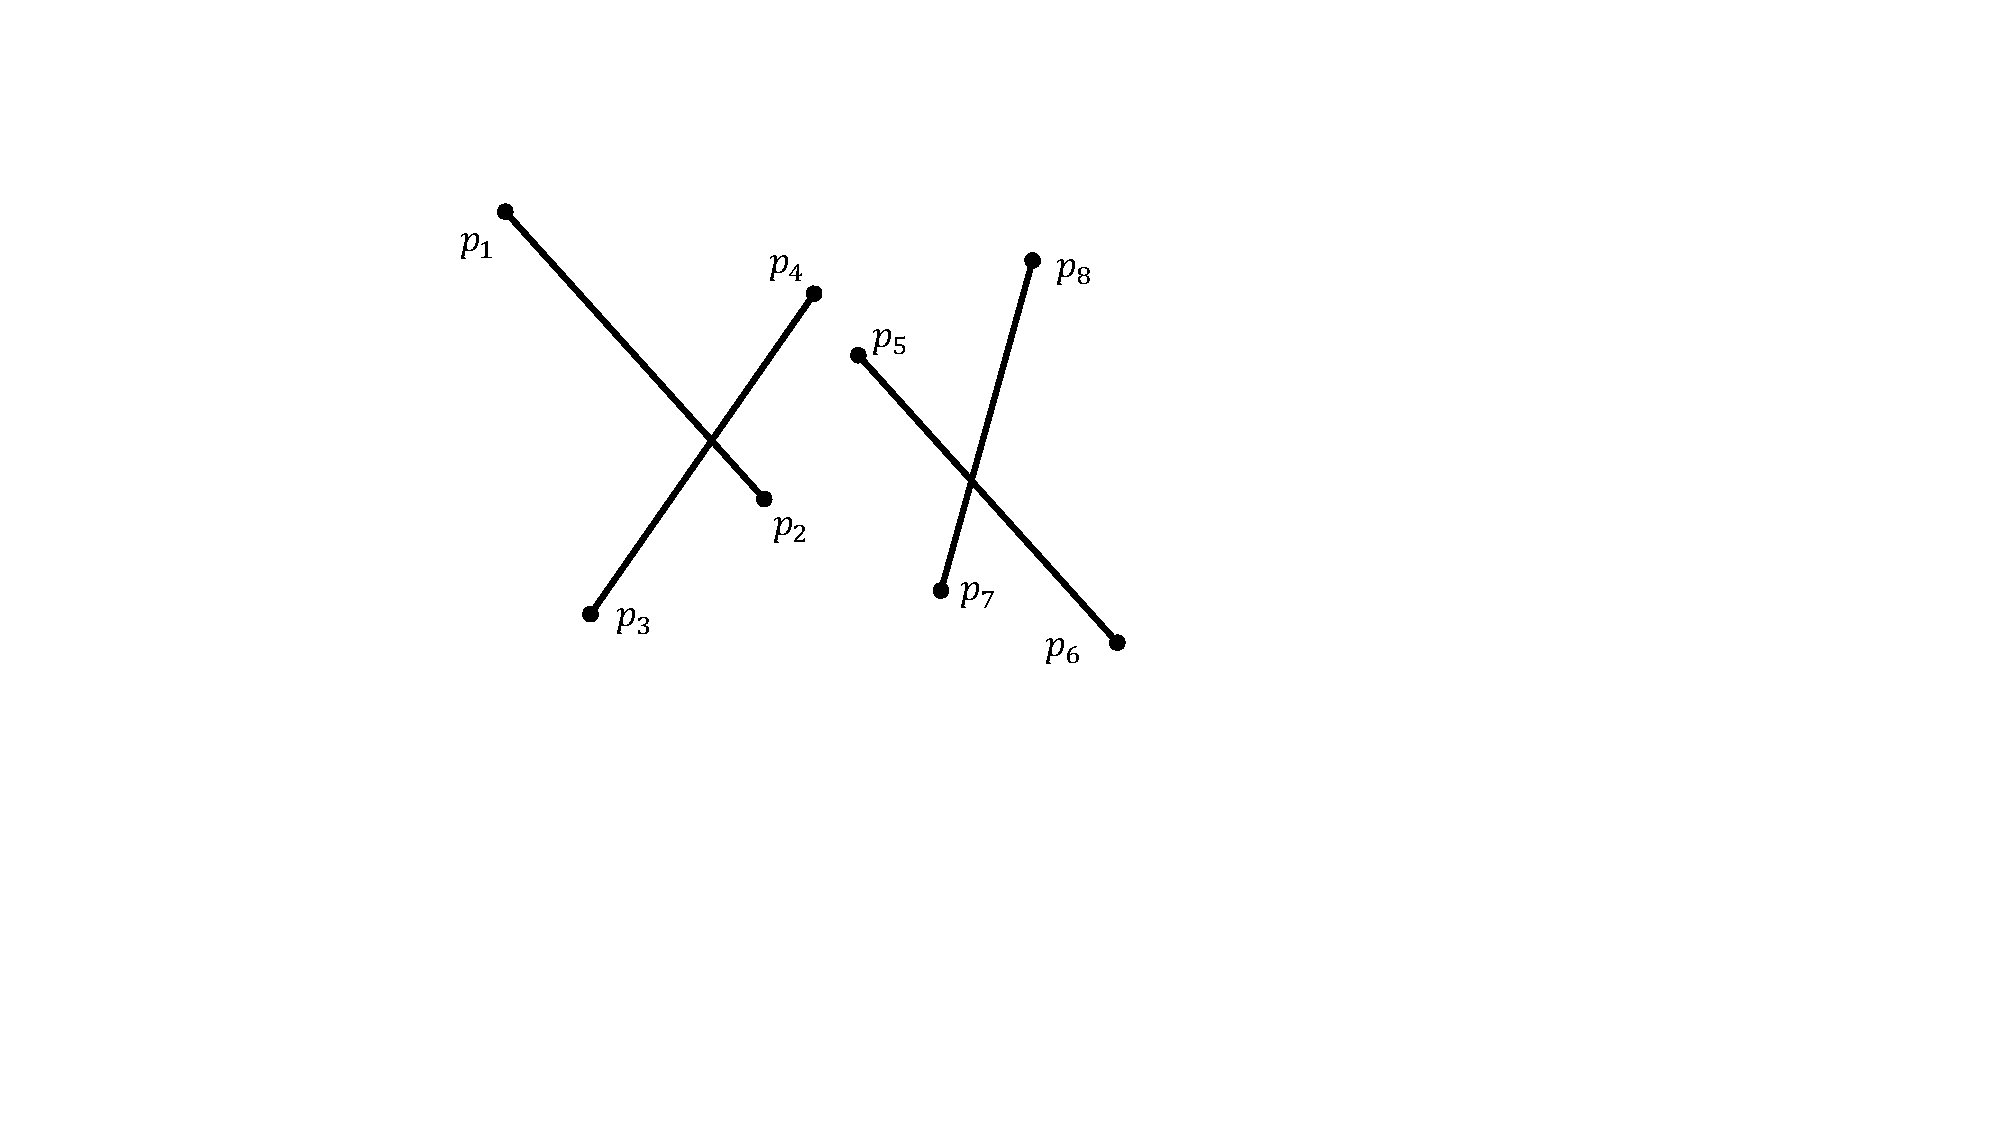
\includegraphics[width=0.7\linewidth]{../images/linesweep.pdf}
\end{center}


\newpage

\begin{tabular}[!h]{|p{6cm}|p{10cm}|}
\hline
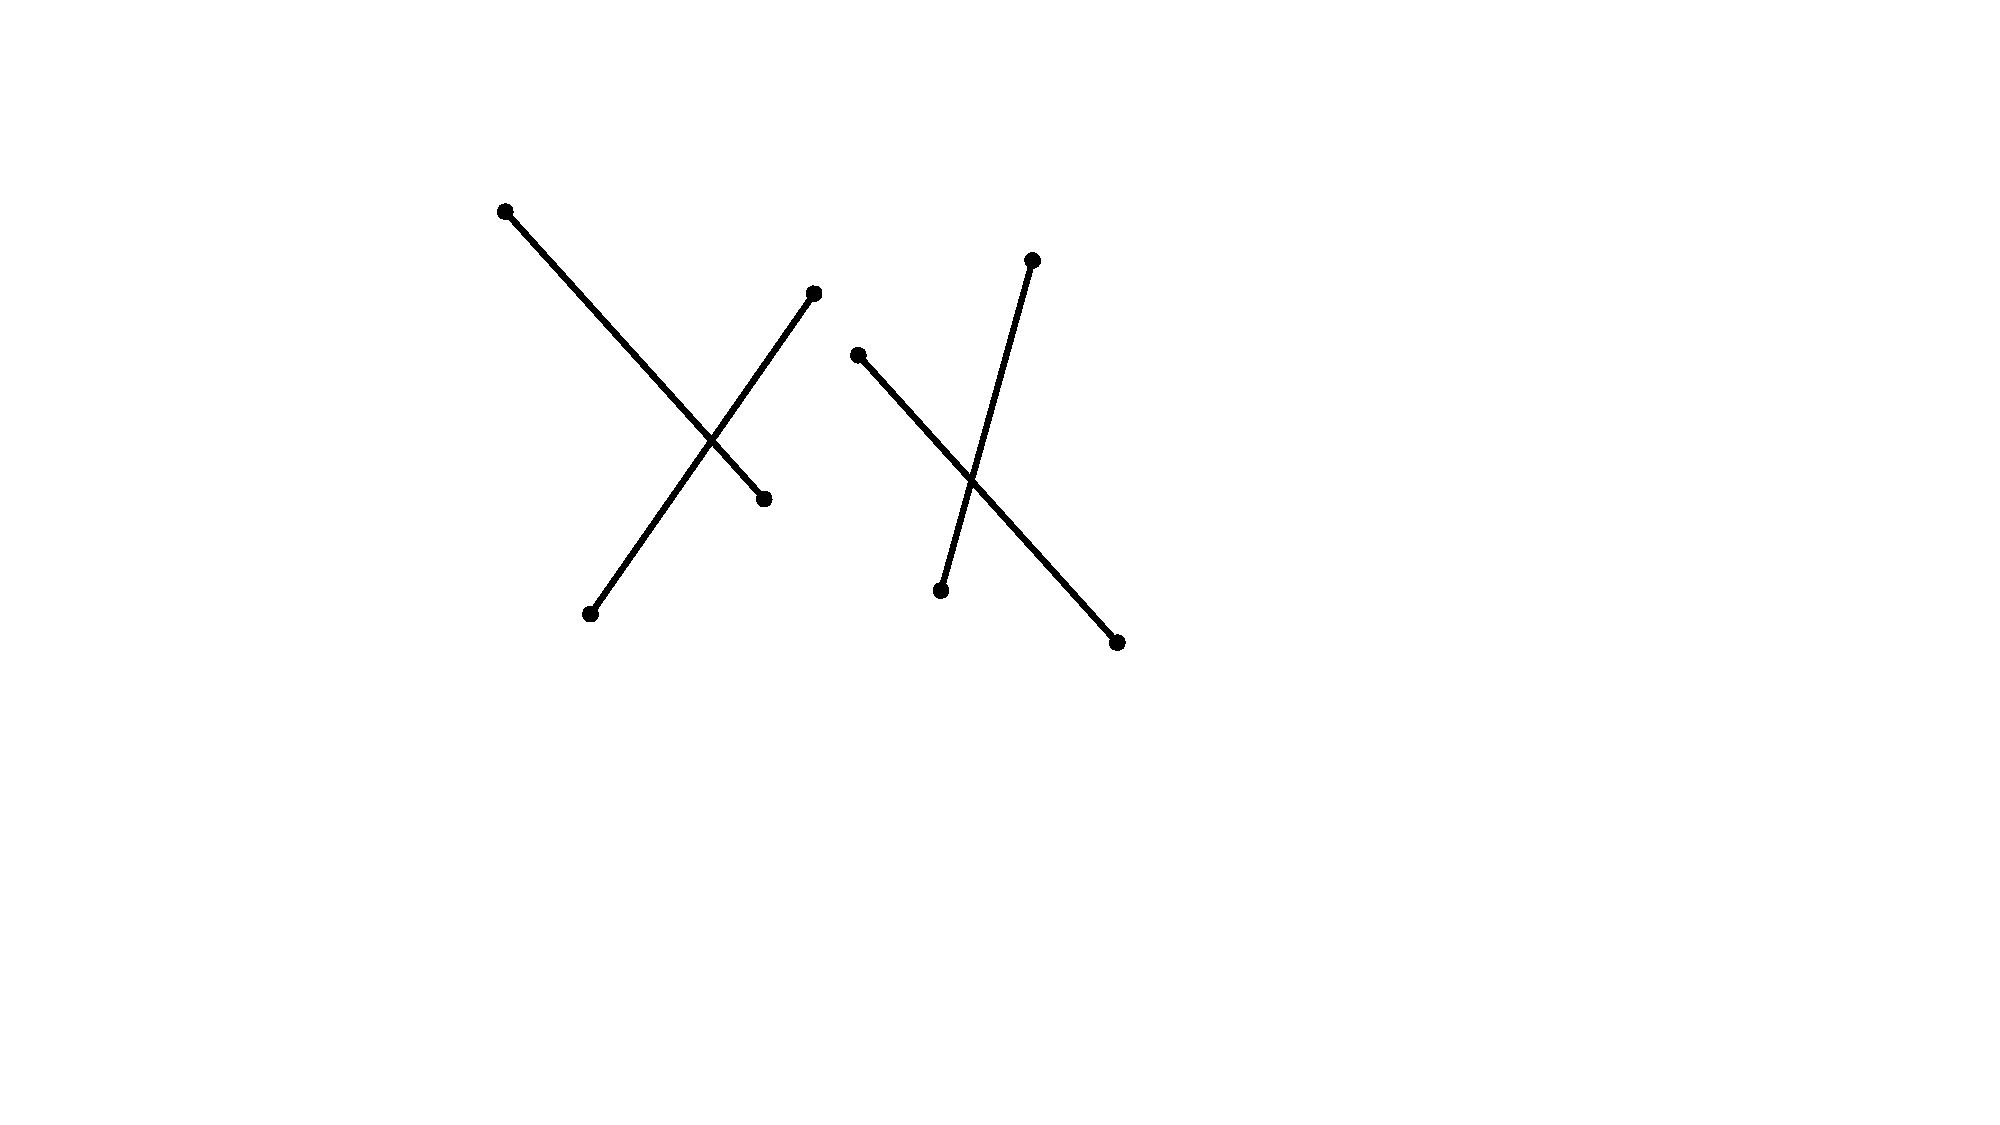
\includegraphics[width=6cm]{../images/linesweep_no_label.pdf} & \\
\hline
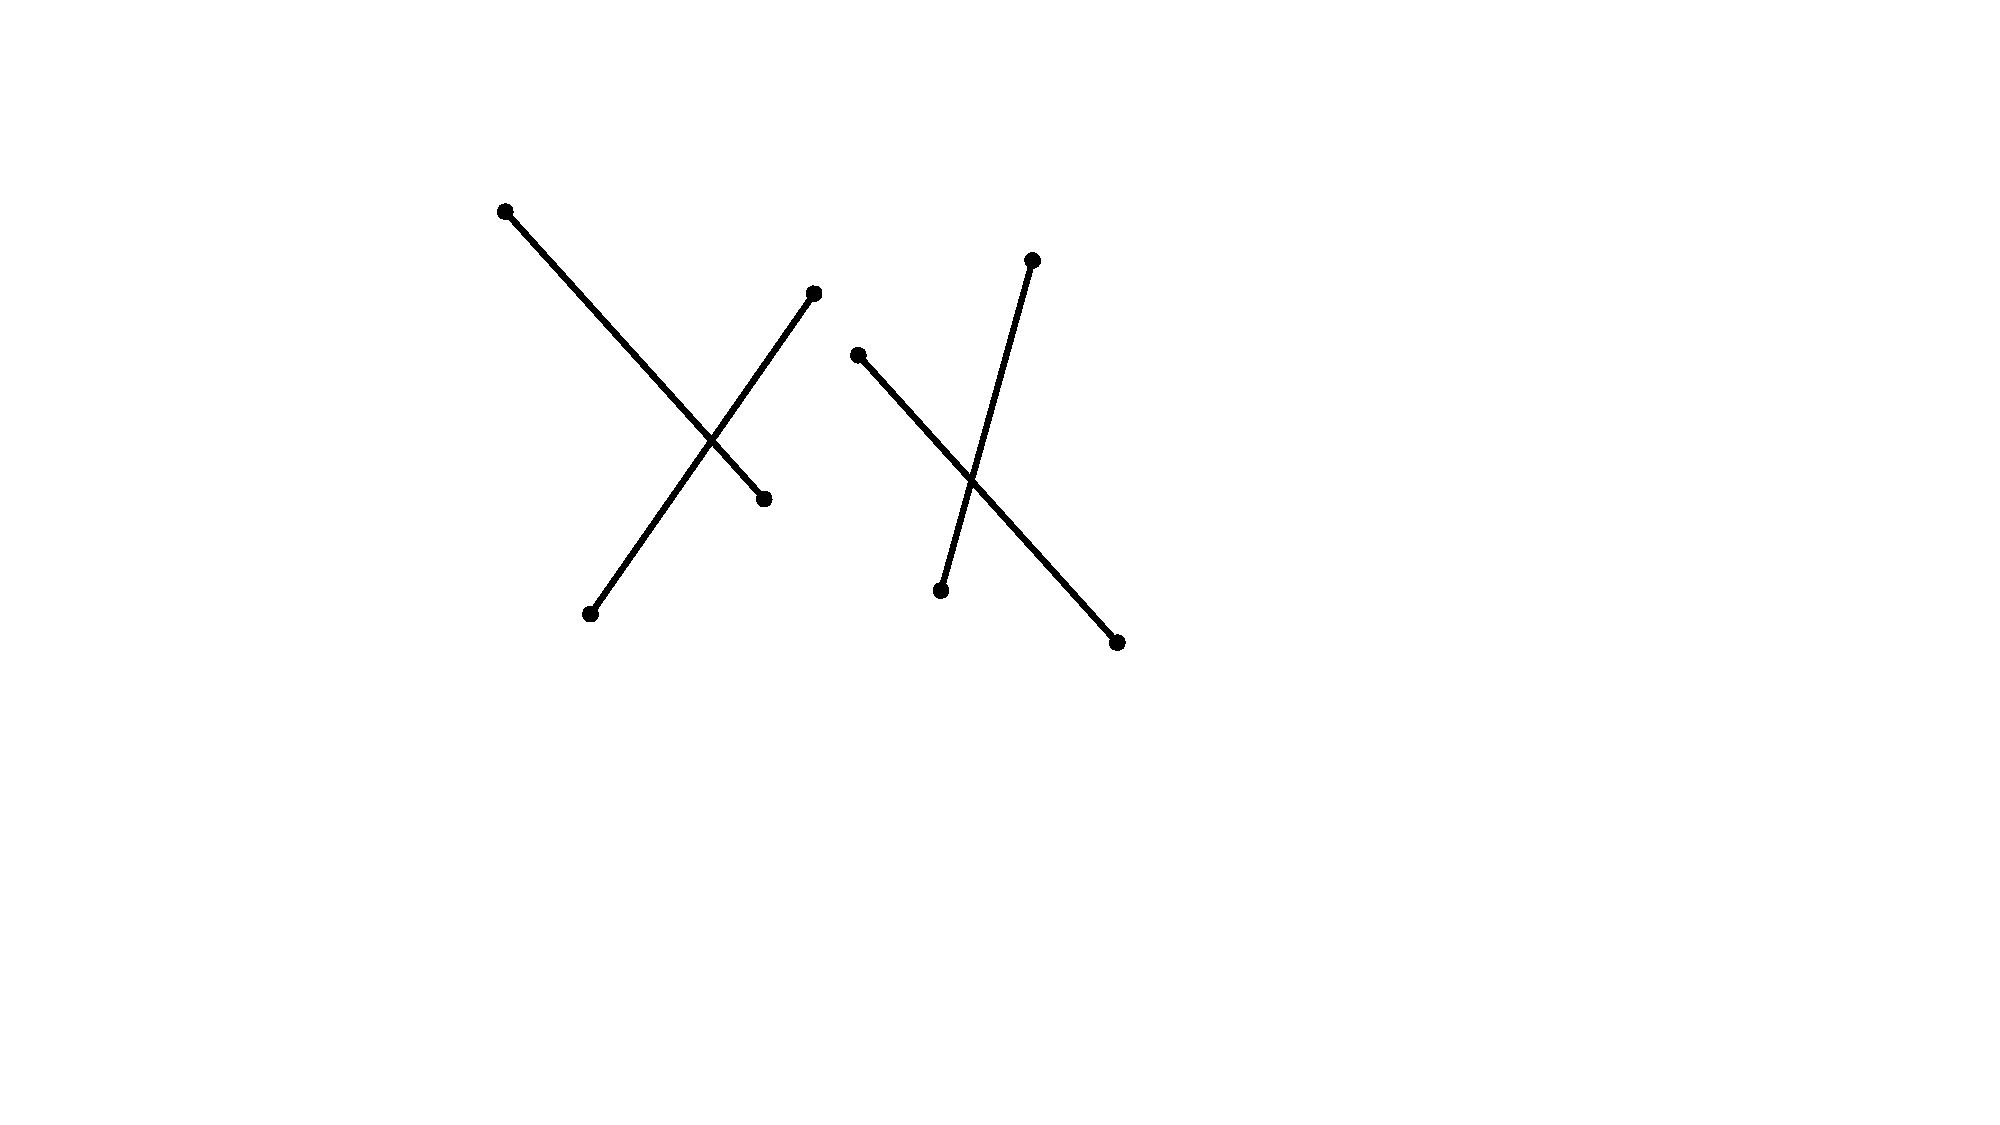
\includegraphics[width=6cm]{../images/linesweep_no_label.pdf} & \\
\hline
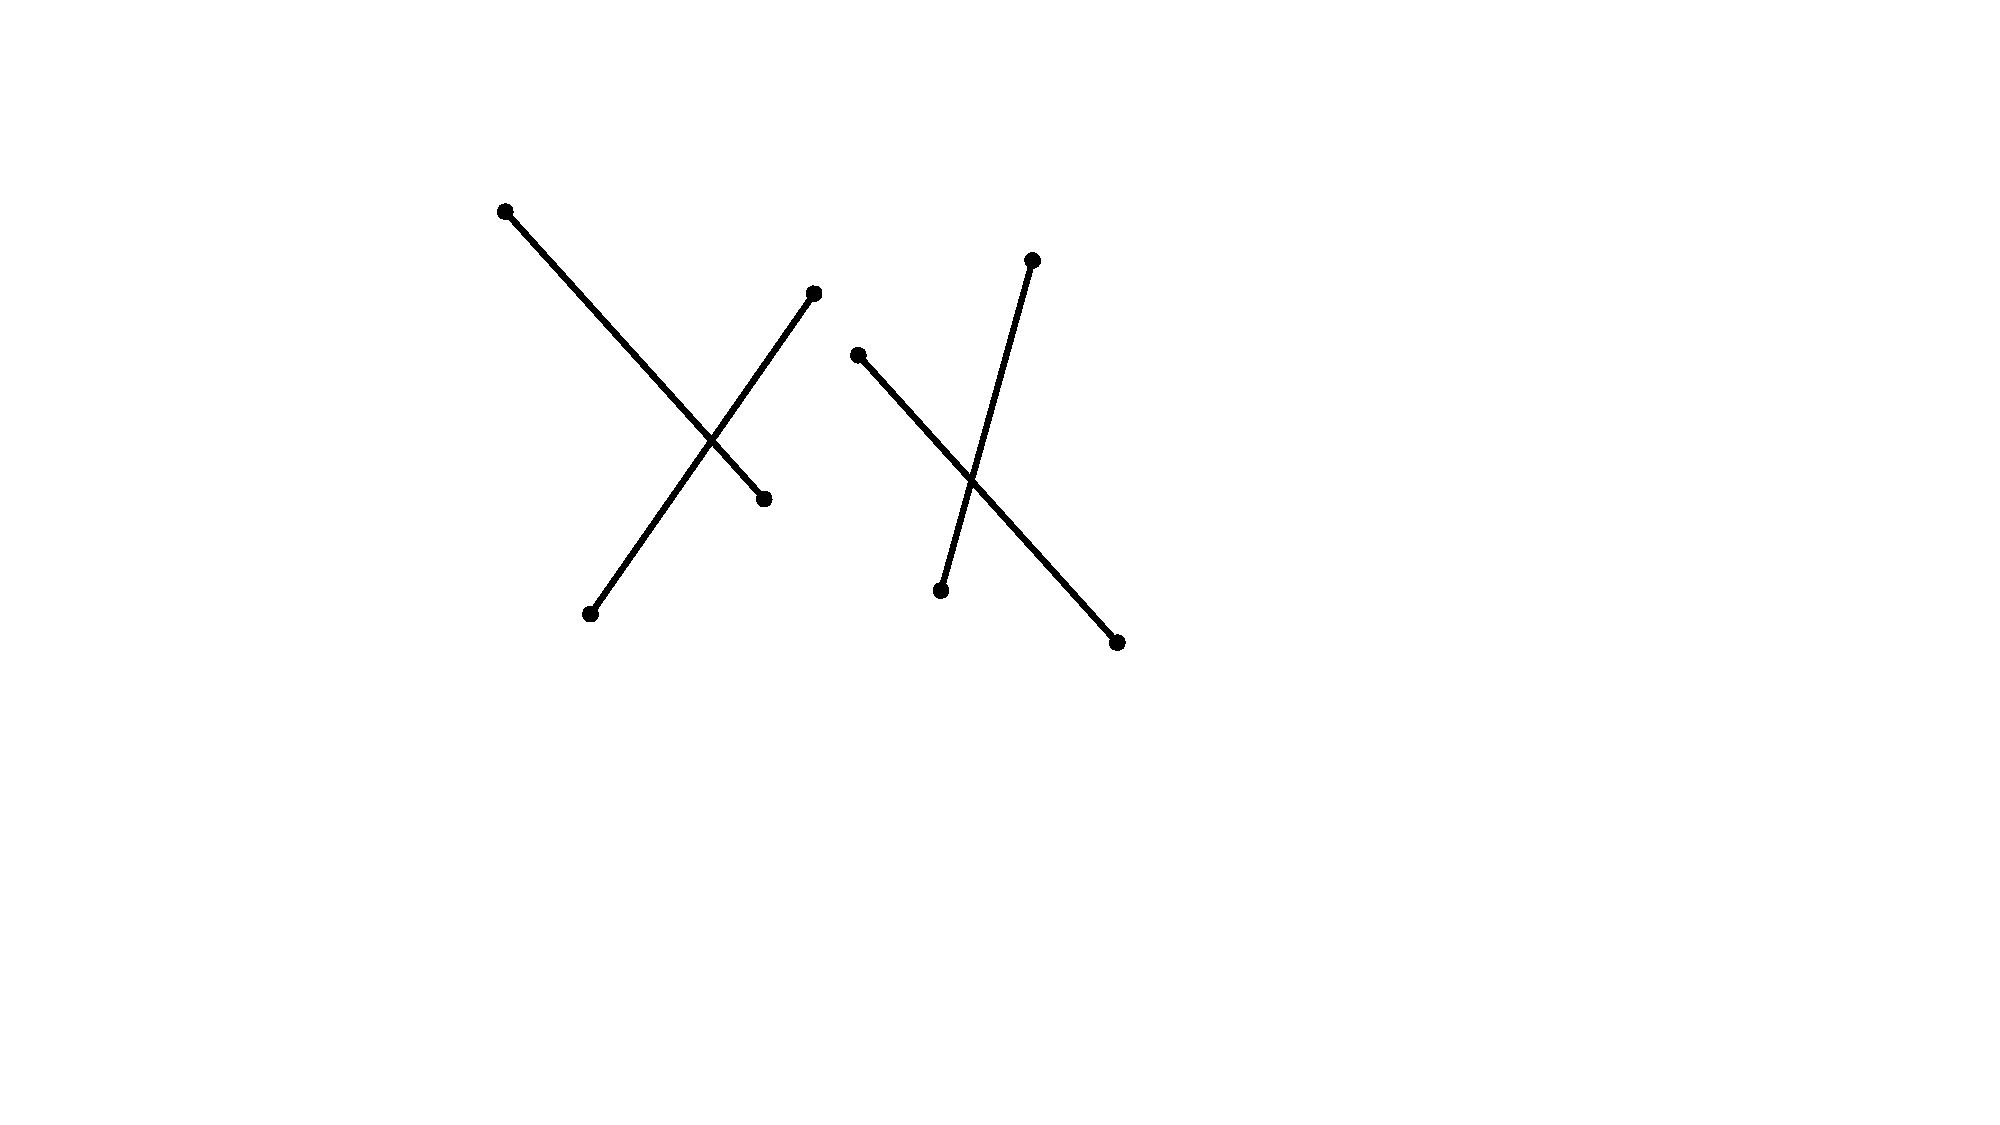
\includegraphics[width=6cm]{../images/linesweep_no_label.pdf} & \\
\hline
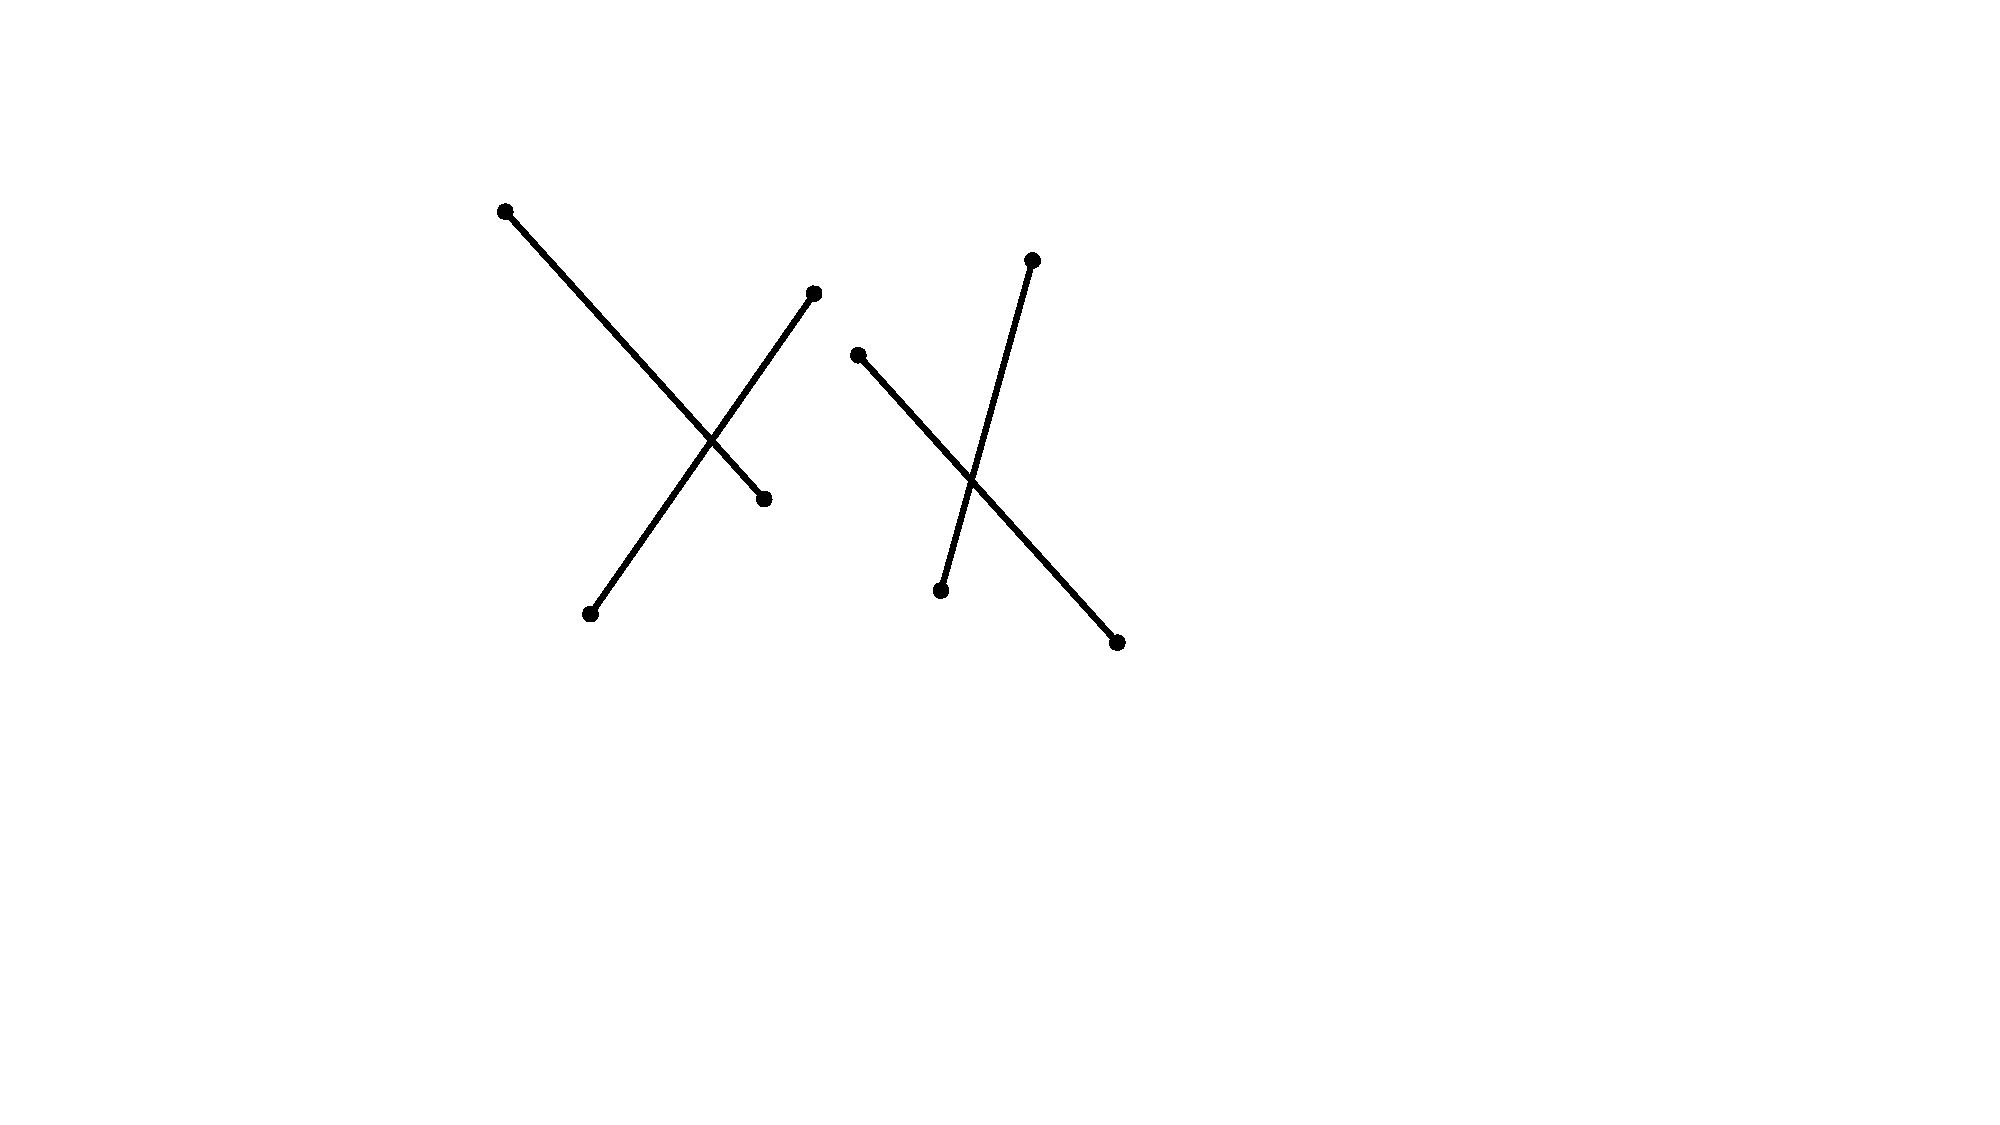
\includegraphics[width=6cm]{../images/linesweep_no_label.pdf} & \\
\hline
\end{tabular}

\begin{tabular}[!h]{|p{6cm}|p{10cm}|}
\hline
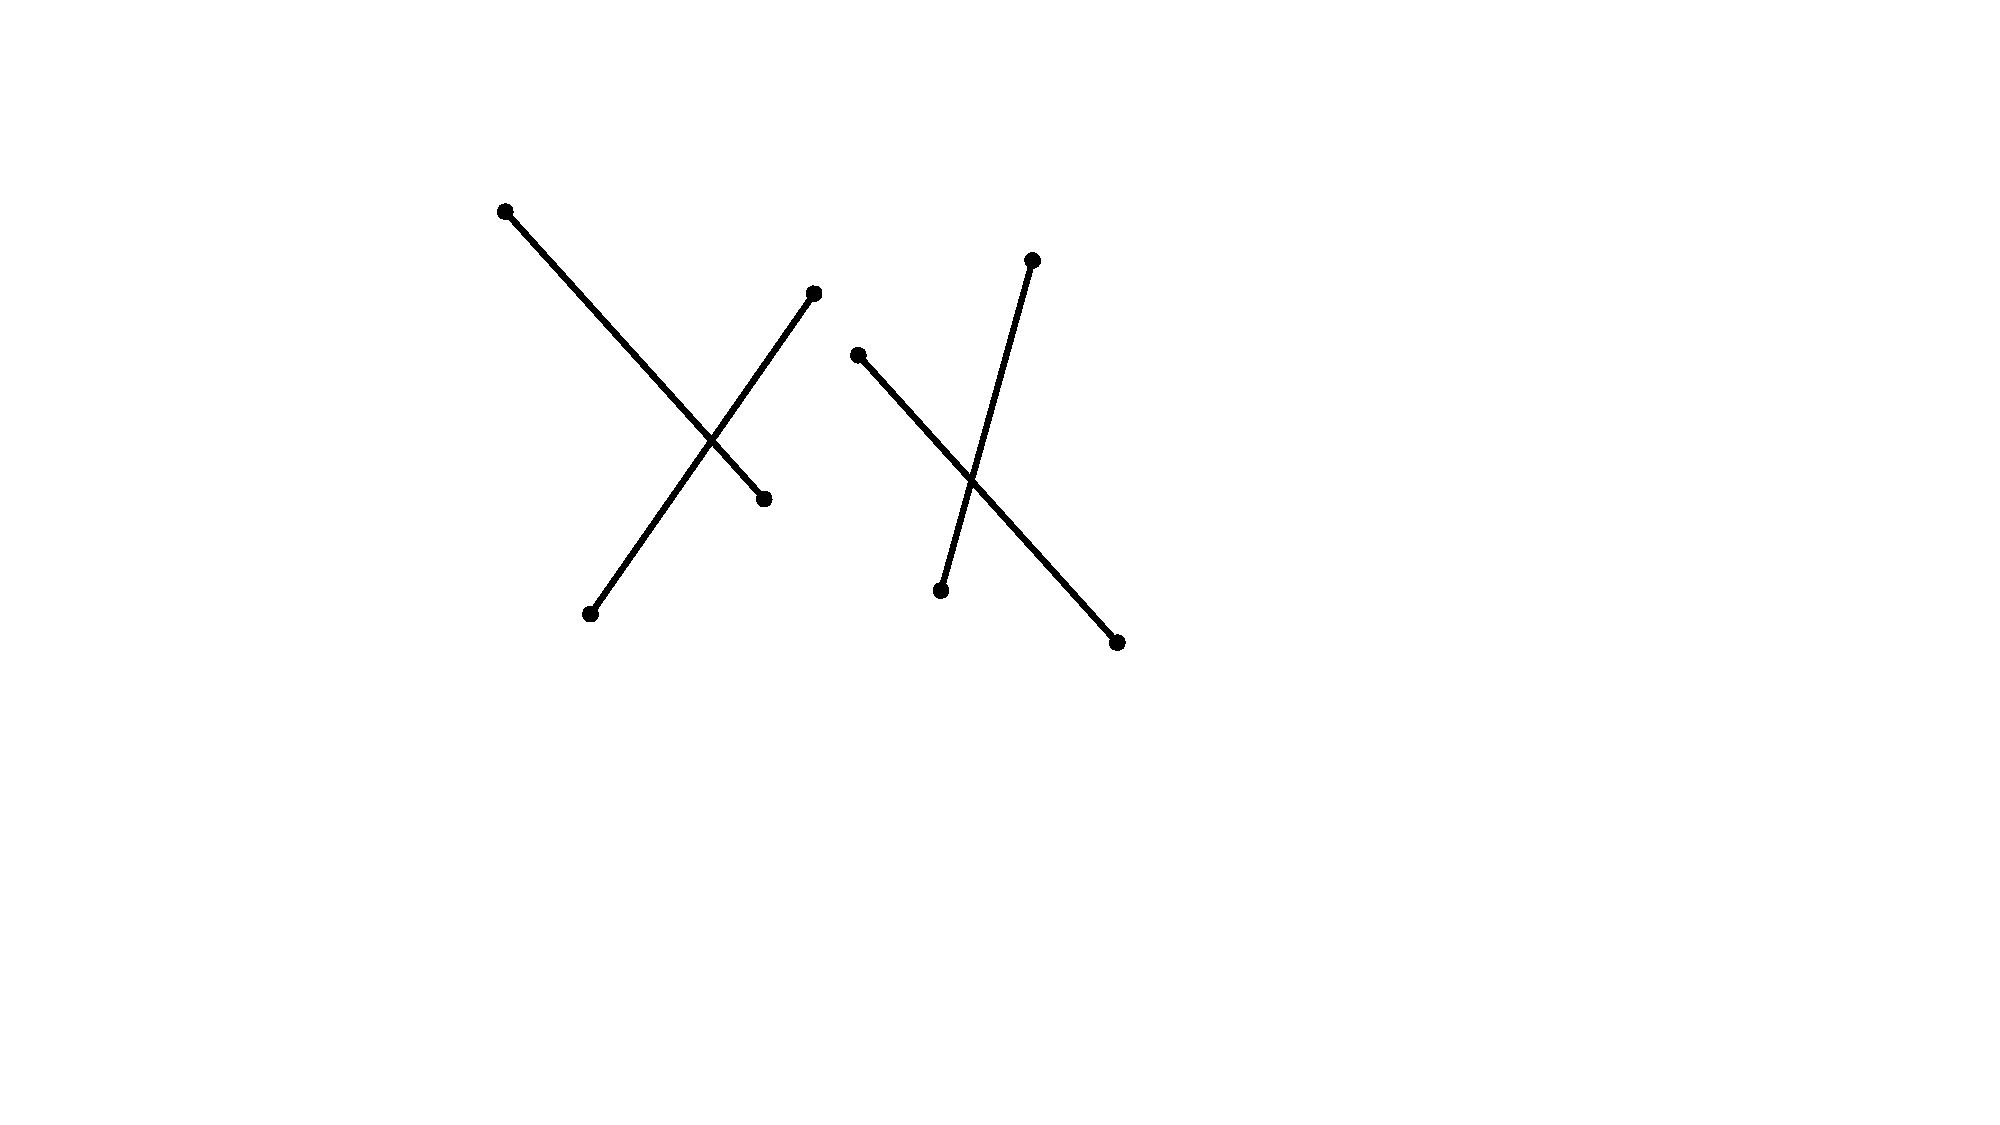
\includegraphics[width=6cm]{../images/linesweep_no_label.pdf} & \\
\hline
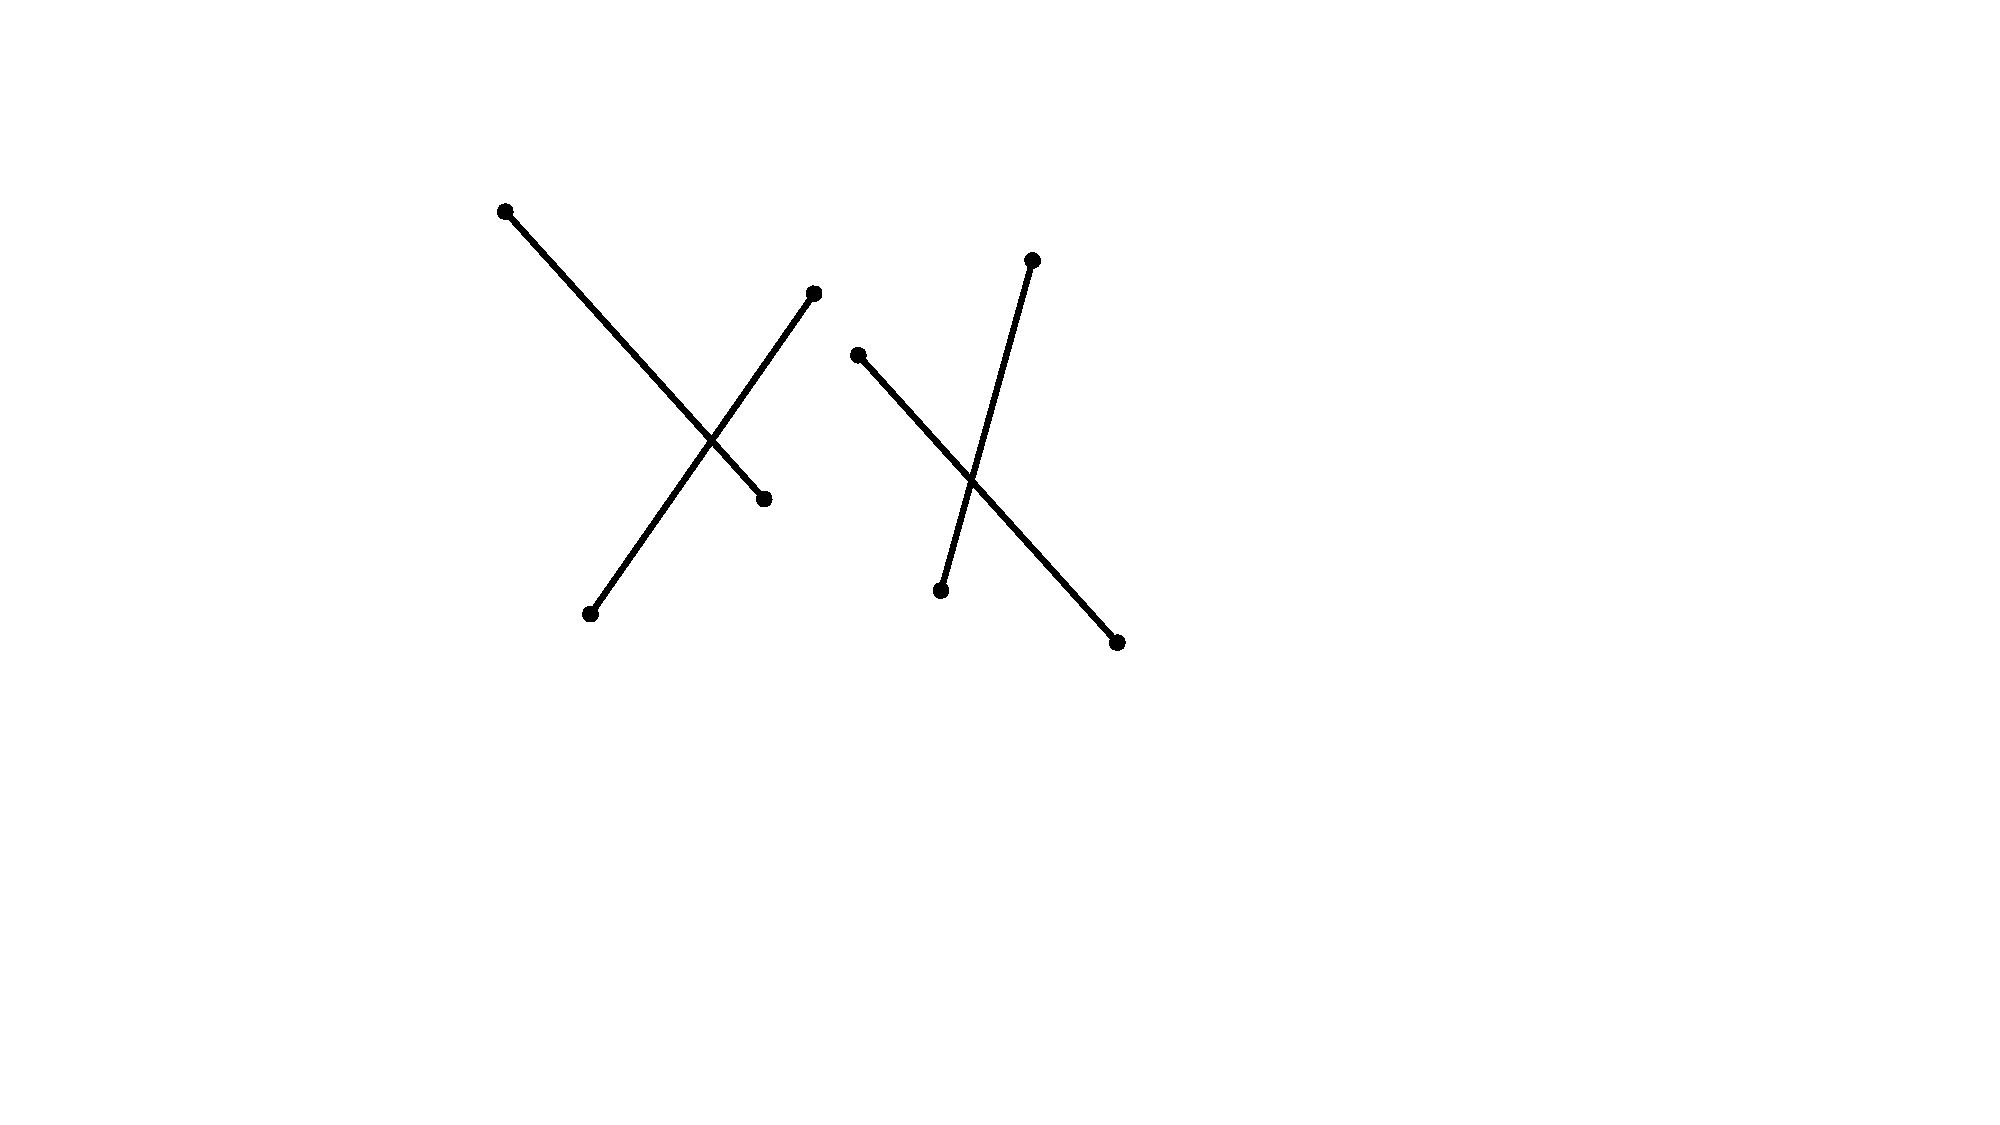
\includegraphics[width=6cm]{../images/linesweep_no_label.pdf} & \\
\hline
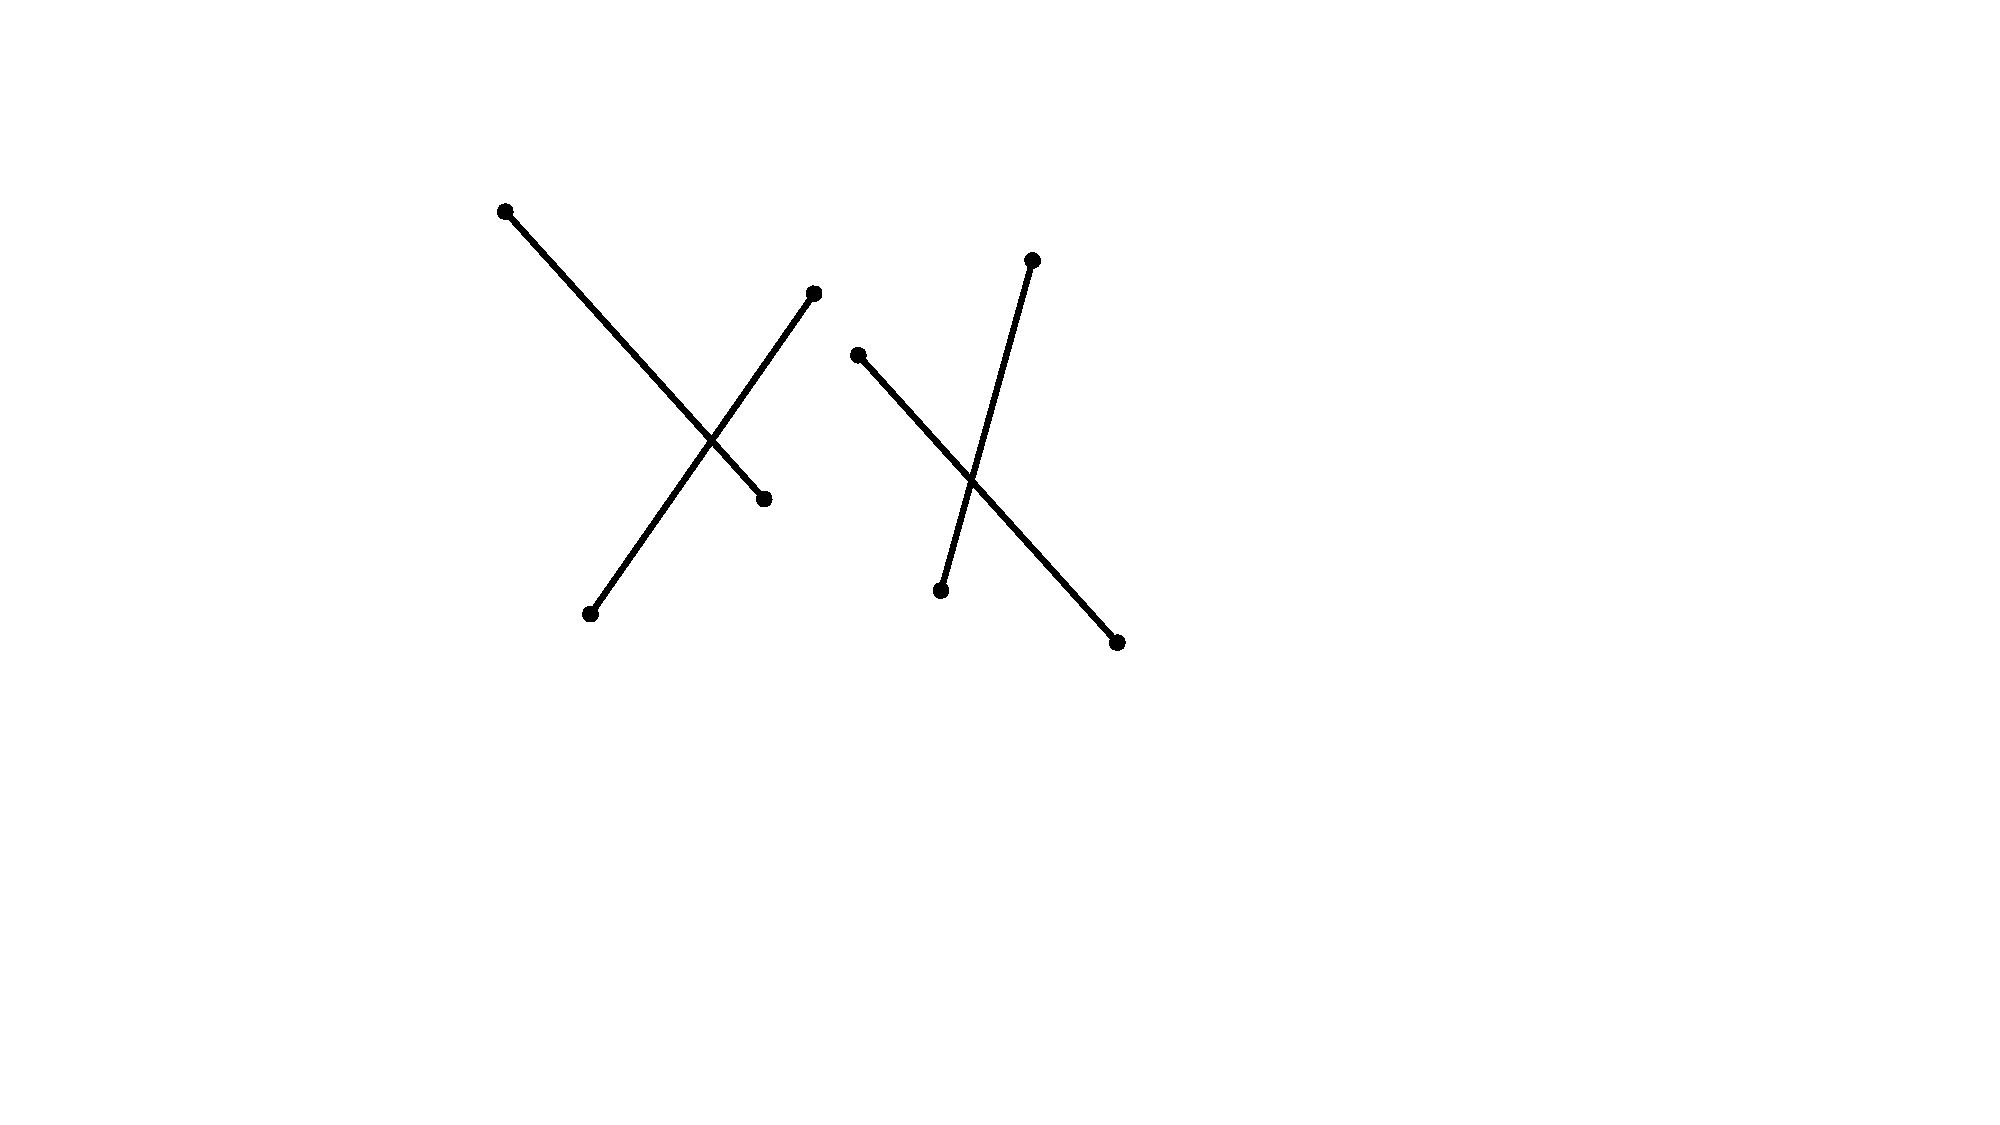
\includegraphics[width=6cm]{../images/linesweep_no_label.pdf} & \\
\hline
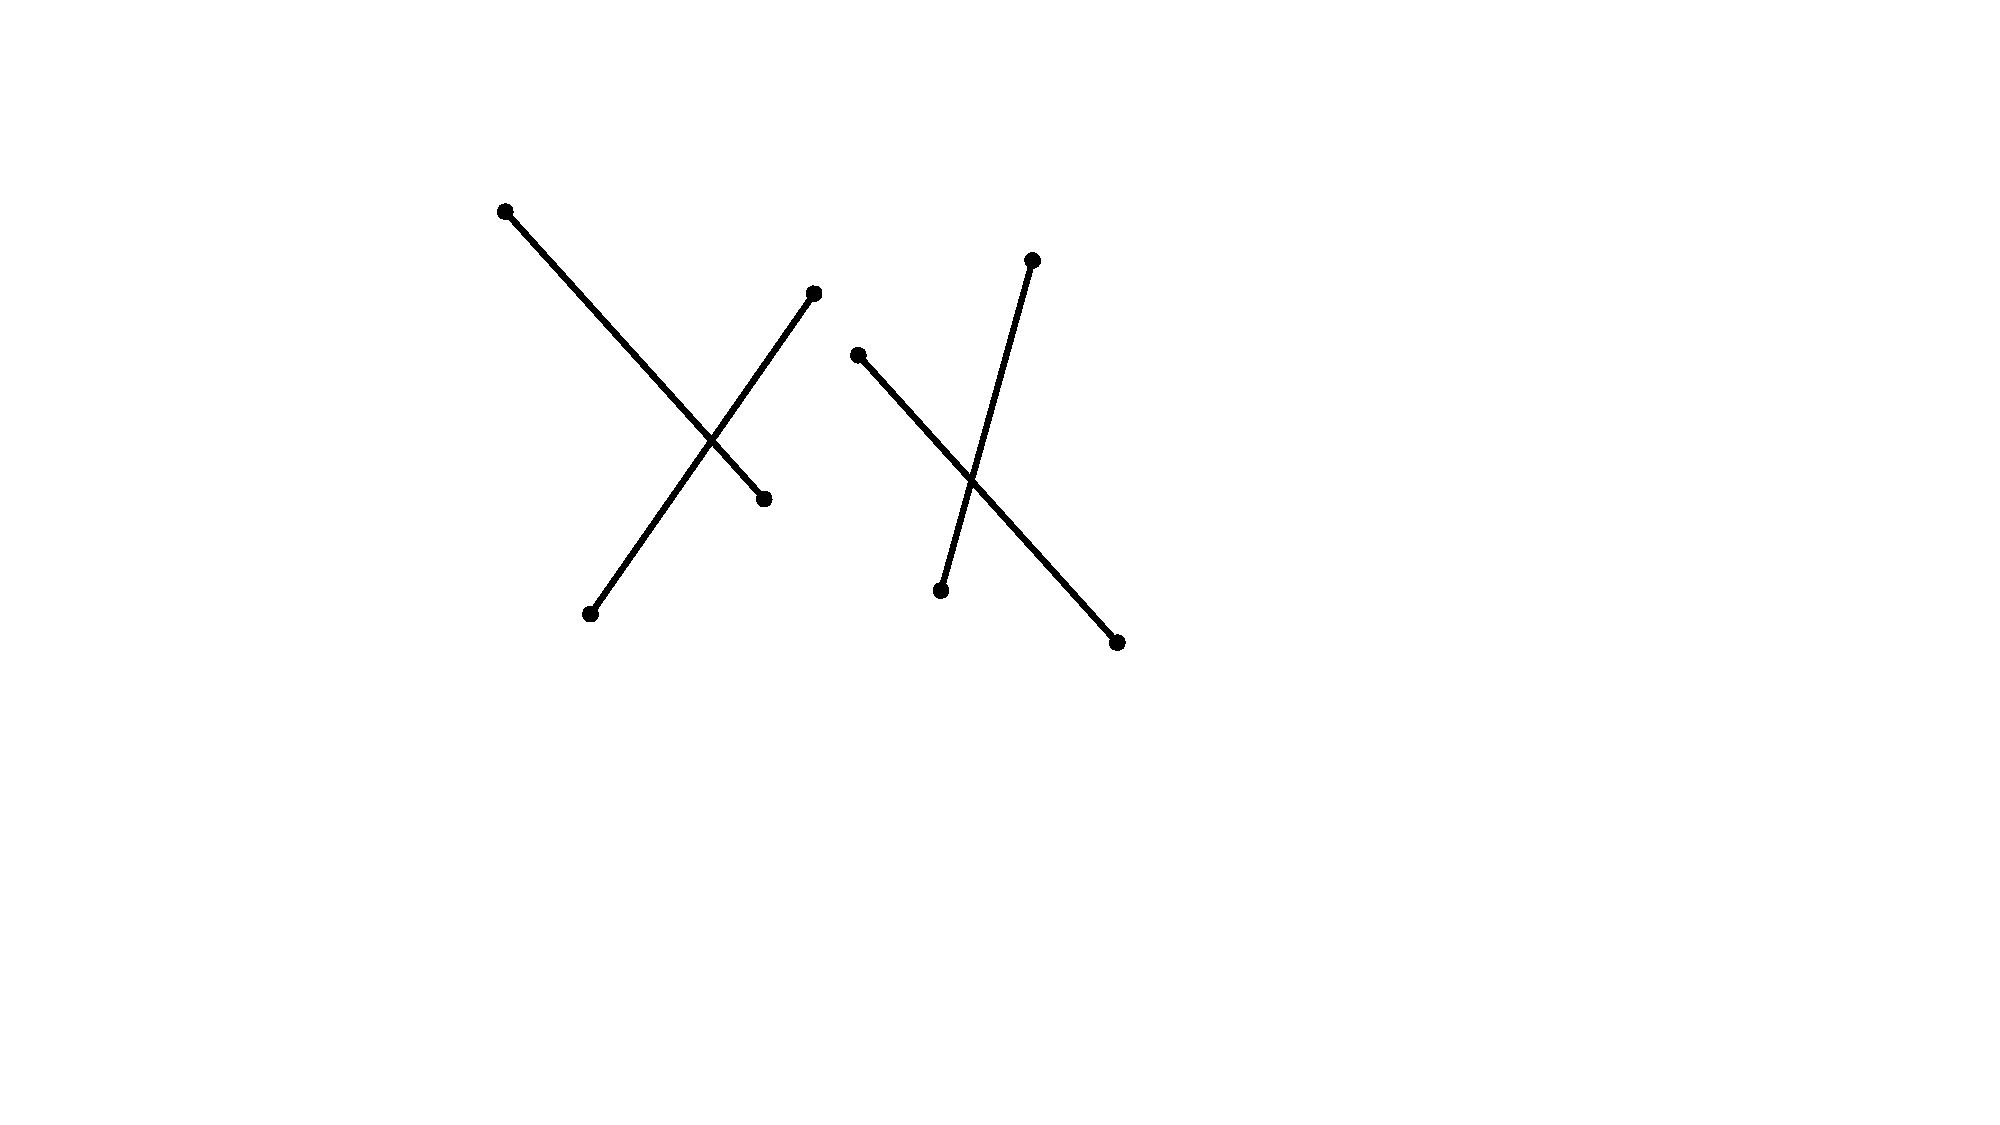
\includegraphics[width=6cm]{../images/linesweep_no_label.pdf} & \\
\hline
\end{tabular}

\end{document}

